\documentclass[8pt]{extarticle}
\title{}
\author{}
\date{}
\usepackage[shortlabels]{enumitem}


%paper setup
\usepackage{geometry}
\geometry{letterpaper, portrait, margin=1in}
\usepackage{fancyhdr}
% sans serif font:
\usepackage{cmbright}
%symbols
\usepackage{amsmath}
\usepackage{bigints}
\usepackage{amssymb}
\usepackage{amsthm}
\usepackage{mathtools}
\usepackage{bbold}
\usepackage[hidelinks]{hyperref}
\usepackage{gensymb}
\usepackage{multirow,array}
\usepackage{multicol}

\newtheorem*{remark}{Remark}
\usepackage[T1]{fontenc}
\usepackage[utf8]{inputenc}

%chemistry stuff
%\usepackage[version=4]{mhchem}
%\usepackage{chemfig}

%plotting
\usepackage{pgfplots}
\usepackage{tikz}
\usetikzlibrary{cd}
\tikzset{middleweight/.style={pos = 0.5}}
%\tikzset{weight/.style={pos = 0.5, fill = white}}
%\tikzset{lateweight/.style={pos = 0.75, fill = white}}
%\tikzset{earlyweight/.style={pos = 0.25, fill=white}}

%\usepackage{natbib}

%graphics stuff
\usepackage{graphicx}
\graphicspath{ {./images/} }
%\usepackage[style=numeric, backend=biber]{biblatex} % Use the numeric style for Vancouver
%\addbibresource{the_bibliography.bib}
%code stuff
%when using minted, make sure to add the -shell-escape flag
%you can use lstlisting if you don't want to use minted
%\usepackage{minted}
%\usemintedstyle{pastie}
%\newminted[javacode]{java}{frame=lines,framesep=2mm,linenos=true,fontsize=\footnotesize,tabsize=3,autogobble,}
%\newminted[cppcode]{cpp}{frame=lines,framesep=2mm,linenos=true,fontsize=\footnotesize,tabsize=3,autogobble,}

%\usepackage{listings}
%\usepackage{color}
%\definecolor{dkgreen}{rgb}{0,0.6,0}
%\definecolor{gray}{rgb}{0.5,0.5,0.5}
%\definecolor{mauve}{rgb}{0.58,0,0.82}
%
%\lstset{frame=tb,
%	language=Java,
%	aboveskip=3mm,
%	belowskip=3mm,
%	showstringspaces=false,
%	columns=flexible,
%	basicstyle={\small\ttfamily},
%	numbers=none,
%	numberstyle=\tiny\color{gray},
%	keywordstyle=\color{blue},
%	commentstyle=\color{dkgreen},
%	stringstyle=\color{mauve},
%	breaklines=true,
%	breakatwhitespace=true,
%	tabsize=3
%}
% text + color boxes
%\renewcommand{\mathbf}[1]{\mathbb{#1}}
%\usepackage[most]{tcolorbox}
%\tcbuselibrary{breakable}
%\tcbuselibrary{skins}
%\newtcolorbox{problem}[1]{colback=white,enhanced,title={\small #1},
%          attach boxed title to top center=
%{yshift=-\tcboxedtitleheight/2},
%boxed title style={size=small,colback=black!60!white}, sharp corners, breakable}
%including PDFs
%\usepackage{pdfpages}
\setlength{\parindent}{0pt}
\usepackage{cancel}
\pagestyle{fancy}
\fancyhf{}
\rhead{Avinash Iyer}
\lhead{Economics of Education: Problem Set 2}
\newcommand{\card}{\text{card}}
\newcommand{\ran}{\text{ran}}
\newcommand{\N}{\mathbb{N}}
\newcommand{\Q}{\mathbb{Q}}
\newcommand{\Z}{\mathbb{Z}}
\newcommand{\R}{\mathbb{R}}
\newcommand{\C}{\mathbb{C}}
\newcommand{\iprod}[2]{\left\langle #1,#2\right\rangle}
\newcommand{\norm}[1]{\left\Vert #1\right\Vert}
\setcounter{secnumdepth}{0}
\begin{document}
\section{Causality in Education}%
\subsection{Problem 1}%
\begin{enumerate}[(a)]
  \item Enrollment in charter schools is often dependent on parental involvement, and higher parental involvement may indicate higher student achievement on principle. Intrinsic student motivation may be different on the basis of their choice to enroll in the public charter school compared to the public school, as well as resources being different between students that choose to attend the public charter school versus the public school. This means that it is likely that the sign of the selection bias is positive --- student achievement is correlated with willingness to enroll in the charter school.\\

    In the potential outcomes framework, we let $S_i$ denote charter vs. public, we let $Z$ denote resources, and we let $P$ denote parental involvement.
    \begin{align*}
      \text{Score}_i &= \alpha_i + \beta_1\text{School Effect}_i + \beta_2\text{Parental Involvement}_i + \beta_3\text{Resources}_i + \varepsilon\\
      \text{OE} &= E(Y_{1i}|S_i=1,Z,P) - E(Y_{0i}|S_i=1,Z,P) + \underbrace{E(Y_{0i}|S_i=1,Z,P)-E(Y_{0i}|S_i=0,Z,P)}_{\text{selection bias}}
    \end{align*}
  \item The size of student loans is correlated with the amount of time spent in education (to an extent), meaning that people who had the capability to work through their education and accrued student loans in the process would also be more likely to be able to manage said student loans once they graduated.
  \item Students at more selective colleges might be able to command other resources such as connections outside the classroom as opposed to pure effect from the quality of education at the college.
  \item Economics majors might be a more affluent cohort than philosophy majors due to holding higher information as to the viability of their major's wage prospects, as well as philosophy majors potentially being willing to take the compensating differential of satisfaction of knowledge over their post-college salary.
\end{enumerate}
\subsection{Problem 2}%
Randomized controlled trials overcome selection bias by removing the ability for participants to select into the treatment or control. However, there are a number of issues with randomized controlled trials:
\begin{itemize}
  \item feasibility: certain experiments are simply impossible to undertake;
  \item ethics: many RCTs have large ethical issues associated with them (including denying agency to those who are subject to them);
  \item external validity: the extent of controls may mean the treatment is not able to be applied to situations not in the experiment.
\end{itemize}
\subsection{Problem 3}%
\begin{enumerate}[(a)]
  \item We view $Q$ as the quantity of teachers in secondary education and $P$ as the wage teachers command.
    \begin{center}
      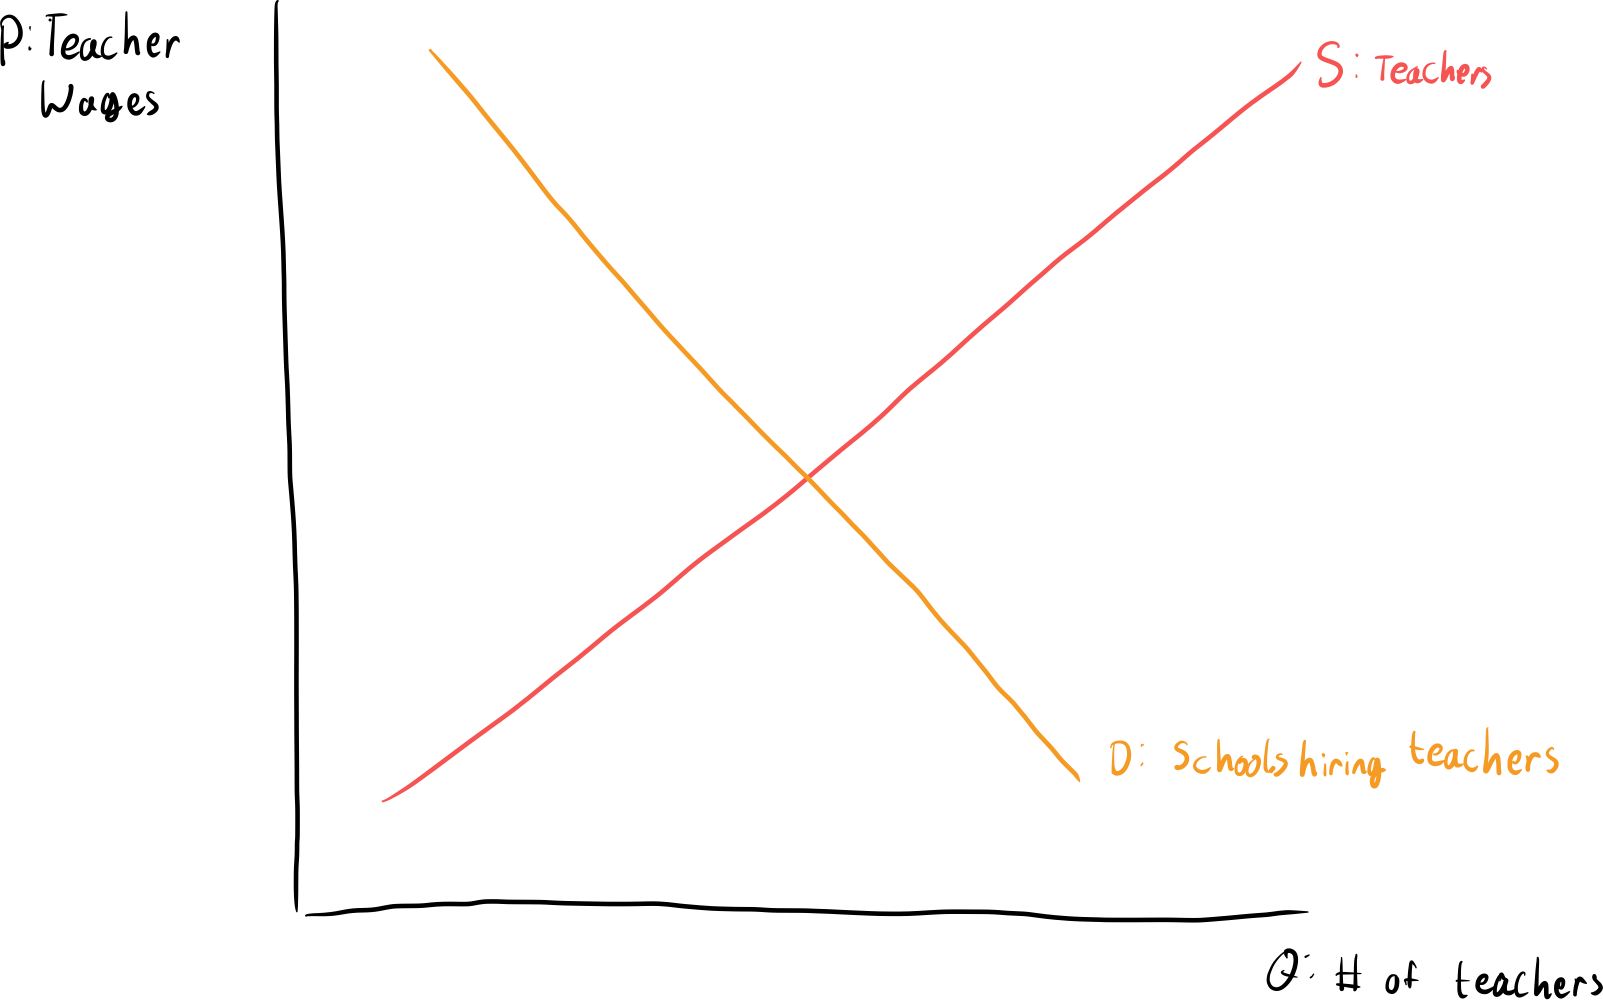
\includegraphics[width=10cm]{images/ps2q3a.png}
    \end{center}
  \item The intersection of supply and demand represent the equilibrium wage of teachers.
  \item If more schools are built we would expect the demand for teachers to increase, leading to an increase in wages and hiring.
    \begin{center}
      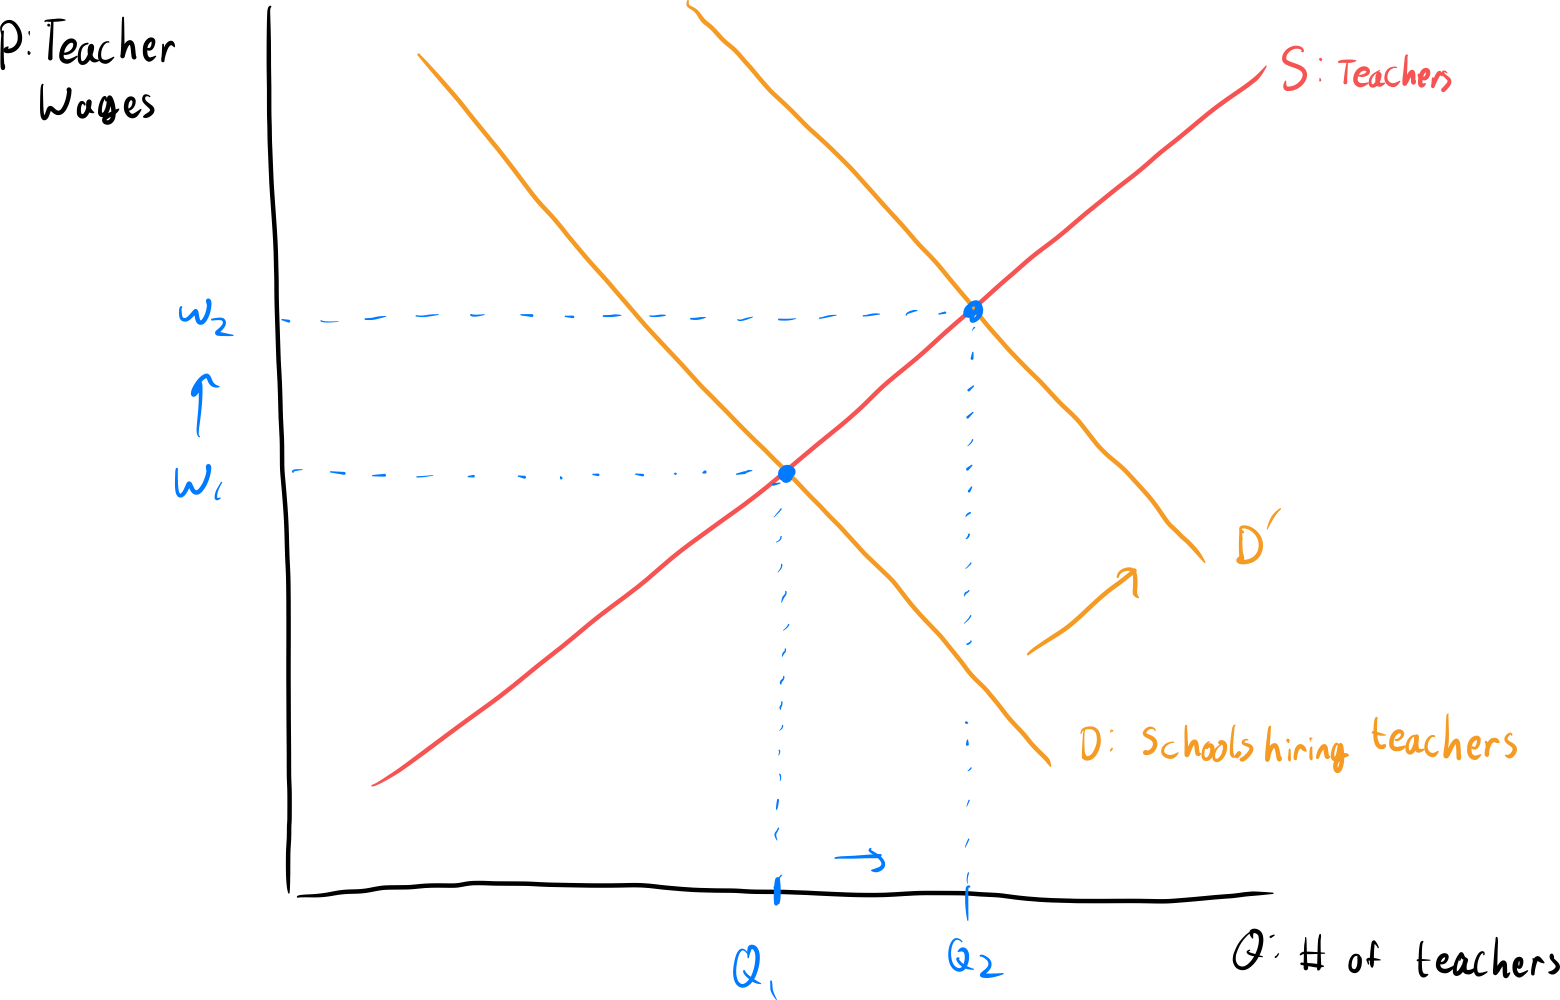
\includegraphics[width=10cm]{images/ps2q3c.png}
    \end{center}
  \item The Roy model predicts that with a relative increase in education premium, the skill of teachers (and the supply of teachers) would decrease. This reduction in barriers to entry would result in a larger supply of teachers, meaning a higher quantity of teachers and lower wages for said teachers.
    \begin{center}
      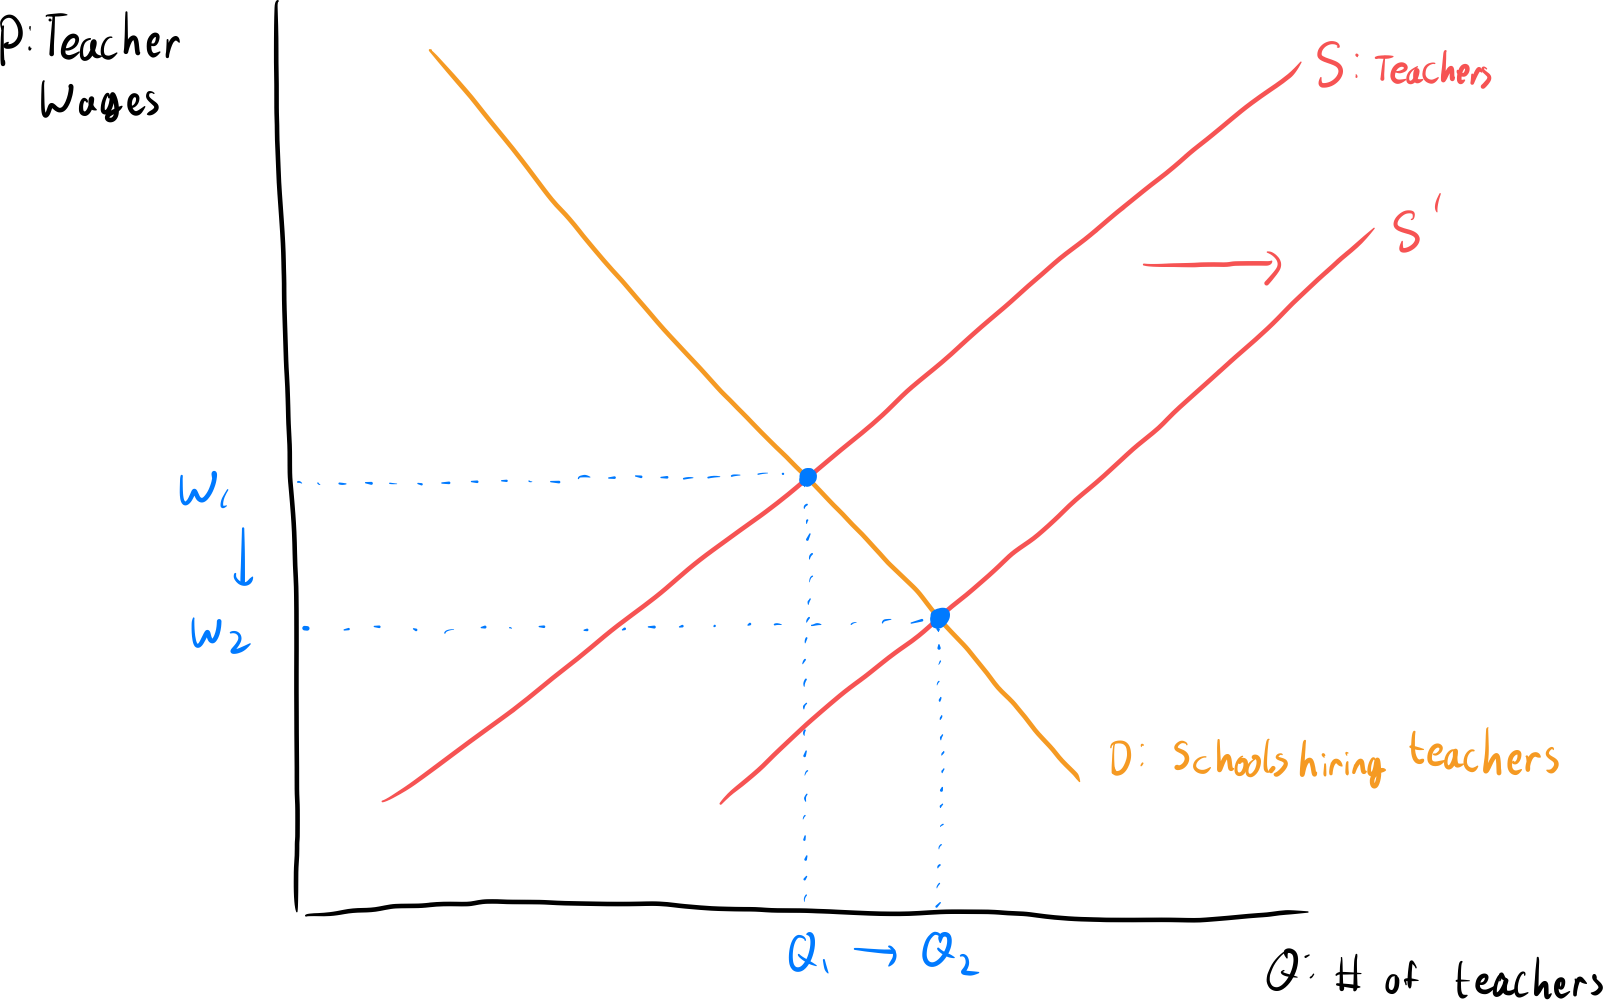
\includegraphics[width=10cm]{images/ps2q3d.png}
    \end{center}
\end{enumerate}
\end{document}
